\chapter{Alpha Particle Formation in Neutron Rich Matter}
One of the triumphs of nuclear physics is the ability to describe properties of macroscopic systems such as neutron stars with microscopic interactions. Neutron stars have been studied extensively with QMC methods, everything from the nuclear EOS (\cite{sarsa2003,gandolfi2014}) to the hyperon problem (\cite{lonardoni2015,gandolfi2018}). As the density of nuclear matter increases the choice of the 3N force becomes more important. However, for neutron star crusts with densities only up to about 0.5$\rho_0$ the choice of 3N force is not as crucial (\cite{gandolfi2009}), and NN forces alone can give good results. The outer crusts of neutron stars host atomic nuclei in a degenerate bath of electrons. As the density increases inside the neutron star the nuclear binding force will eventually give way to neutron drip and the remaining nuclei will be in a fluid of dripped neutrons. This has been studied (\cite{lorenz1993,chamel2015}) and the density at which neutron rich nuclei begin to drip neutrons is about $\rho_\text{drip} = 4.3\times10^{11}$ g cm$^{-3}$ or 0.00026 fm$^{-3}$. This neutron drip will leave smaller and smaller nuclei in a sea of neutrons. At high enough density all nuclei will dissolve to form uniform neutron matter, or mostly-neutron matter. To investigate this transition I have studied the formation of alpha particles in mostly-neutron matter. To do this I have used the AFDMC method in conjunction with the AV6$'$ potential using both the linear and quadratic trial wave functions. The energy of an alpha particle that has formed in neutron matter with an additional two protons would be
\begin{equation}
   E_\alpha = E_\text{Nn2p} - E_\text{N-2n},
   \label{equ:alphaenergy}
\end{equation}
where $E_\text{Nn2p}$ is the energy for $N$ neutrons and 2 protons and $E_\text{N-2n}$ is the energy for $N-2$ neutrons alone. Protons and neutrons can exchange a charged pion, effectively changing $pn$ to $np$. As a result, we cannot assign the label of proton or neutron to any particular particle, and thus all particles must be antisymmetrized together. I have calculated the energy per particle of 14 neutrons with and without the presence of 2 protons in a box with periodic boundary conditions. At appropriate densities the 2 protons will form, with 2 neutrons, an alpha particle surrounded by free neutrons. I am calling the energy of the 2 protons and 2 neutrons the alpha particle energy, $E_\alpha$ as given by Equation~\ref{equ:alphaenergy} regardless of whether the alpha particle is formed or not. For 14 neutrons and 2 protons this is calculated as
\begin{equation}
   E_\alpha = E_\text{14n2p} - E_\text{12n}.
\end{equation}
In practice we calculated the energy per particle with 14 neutrons instead of 12. The plane wave shell is filled with 14 neutrons, 7 with spin up, and 7 with spin down, making the calculation easier with 14 neutrons. As a result, if the energy per particle is given by $\epsilon = E/A$ then in practice the alpha particle energy is calculated as
\begin{equation}
   E_\alpha = 16\epsilon_\text{14n2p} - 12\epsilon_\text{14n}.
   \label{equ:alphaenergy14n2p}
\end{equation}

The single particle states used for all nuclear matter calculations in the work are plane waves multiplied by appropriate spin-isospin states,
\begin{equation}
   \phi_\alpha(\r_i,s_i) = e^{\mathbf{k}_\alpha\cdot\r_i}\braket{\chi_{s,m_s}}{s_i},
\end{equation}
where the possible $\mathbf{k}$ vectors are given by
\begin{equation}
   \mathbf{k}_\alpha = \frac{2\pi}{L}(n_{x\alpha},n_{y\alpha},n_{z\alpha}).
\end{equation}
Periodic boundary conditions are used to help reduce finite-size effects and assume that an exact copy of the wave function repeats across the simulation boundary,
\begin{equation}
   \psi(\r_i+L\hat{\mathbf{x}}) = \psi(\r_i).
\end{equation}

Ideally it would be better to do calculations with different numbers of neutrons, however 14 neutrons fills a plane wave shell as defined by the possible $(n_{x},n_{y},n_{z})$ with both spin up and spin down neutrons and the next smallest plane wave shell would contain 38 neutrons. This calculation is possible but is much larger and prohibitively expensive to repeat many times with quadratic correlations. As will be discussed shortly the underbinding at low densities would probably be exaggerated with a larger fraction of neutrons in the calculation, though additional neutrons will have a smaller effect due to the short range of the nuclear interaction. It is possible to use numbers of neutrons between closed shells by using larger numbers of determinants, however that also becomes too expensive. It could be possible to include intermediate numbers of neutrons by using twist instead of periodic boundary conditions (\cite{lin2001}). The twist boundary conditions are a generalization to the periodic boundary conditions mentioned previously and are written as
\begin{equation}
   \psi(\r_i+L\hat{\mathbf{x}}) = e^{i\theta}\psi(\r_i),
\end{equation}
where $\theta=0$ gives periodic boundary conditions and $\theta\ne0$ gives the twist boundary condition. The twist angle, $\theta$, is integrated over, which effectively reduces the finite-size effects coming from filled plane-wave shells. This effectively allows states that wouldn't fit in the typical closed shells and reduces the effects of having a hard shell structure. One way to do this as described in \cite{gandolfi2009} is to define different $\mathbf{k}_i$ vectors as
\begin{equation}
   \mathbf{k}_{\alpha,i} = (2\pi\mathbf{n}_\alpha + \theta_i)/L.
\end{equation}
A separate simulation is performed for each twist angle and the energies for each calculations are averaged to obtain the final energy. This is a possible extension to the current work.

I have plotted the alpha particle energy as a function of density using both linear and quadratic correlations in Figure~\ref{fig:alpha}.
\begin{figure}[h!]
   \centering
   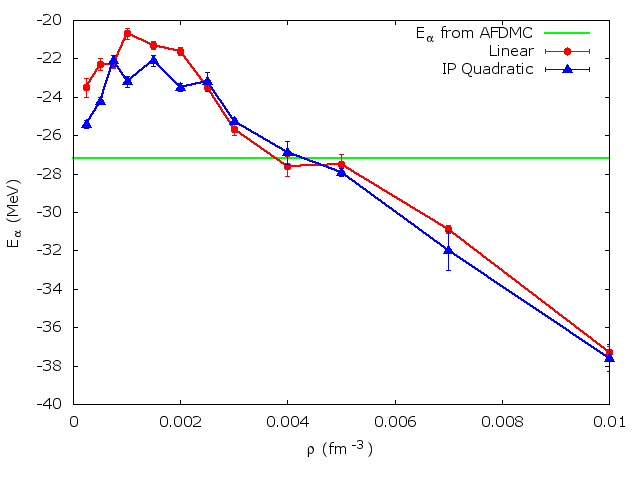
\includegraphics[width=0.7\textwidth]{figures/alpha.png}
   \caption[Energy of 2 Protons and 2 Neutrons with 12 Free Neutrons as Calculated with Equation~\ref{equ:alphaenergy14n2p} as Calculated with Linear and Quadratic Correlations. The Green Horizontal Line Indicates the Alpha Particle Energy as Calculated with AFDMC Using the Same AV6$'$ Interaction and Quadratic Correlations.]{Energy of 2 protons and 2 neutrons with 12 free neutrons as calculated with Equation~\ref{equ:alphaenergy14n2p} as calculated with linear and quadratic correlations. The green horizontal line indicates the alpha particle energy as calculated with AFDMC using the same AV6$'$ interaction and quadratic correlations.}
   \label{fig:alpha}
\end{figure}
If the free neutrons did not interact with the formed alpha particle it would be expected that the alpha particle energy would agree with previous AFDMC calculations, the results of which are indicated with a green horizontal line. At densities below 0.0025 fm$^{-3}$ the alpha particle is underbound by a few MeV for both linear and quadratic correlations. The quadratic correlations do decrease the alpha energy at low densities. Previously I showed that the quadratic correlations had very little effect on the energy of an alpha particle and so the difference in energy for the linear and quadratic correlations must be related to the alpha-neutron interactions. In addition, the energy for each individual calculation of $E_\text{14n2p}$ and $E_\text{12n}$ were decreased with quadratic correlations with respect to linear correlations. The difference between quadratic and linear correlations seems to be the most important for most densities below 0.0025 fm$^{-3}$.

The discrepancy in alpha particle energy at low densities must be due to the excess neutrons deforming the alpha particle. To verify that 2 protons and 2 neutrons, without any free neutrons, will give the correct energy in a periodic box I have calculated the energy of 2 protons and 2 neutrons in various boxes of different densities as shown in Figure~\ref{fig:alpha2n2p}.
\begin{figure}[h!]
   \centering
   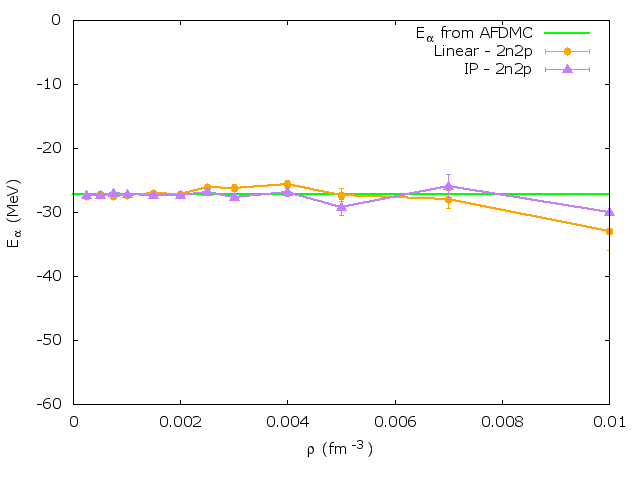
\includegraphics[width=0.7\textwidth]{figures/2n2p.png}
   \caption[Energy of 2 Protons and 2 Neutrons as Calculated with Linear and Quadratic Correlations. The Green Horizontal Line Indicates the Alpha Particle Energy as Calculated with AFDMC Using the Same AV6$'$ Interaction and Quadratic Correlations.]{Energy of 2 protons and 2 neutrons as calculated with linear and quadratic correlations. The green horizontal line indicates the alpha particle energy as calculated with AFDMC using the same AV6$'$ interaction and quadratic correlations.}
   \label{fig:alpha2n2p}
\end{figure}
The energy at low densities is much closer to the alpha particle energy as calculated with AFDMC.

The other possible explanation for the underbinding of the 4 nucleons at low density is that the alpha particle doesn't form at all. To investigate this I have looked at the pair correlations function
\begin{equation}
   g_\mathcal{O}(r) = \frac{1}{4\pi r^2} \bra{\Psi}\sum\limits_{i<j}\mathcal{O}_{ij}\delta(r-r_{ij})\ket{\Psi},
\end{equation}
where I have specifically looked at the case where the operator is the $pp$ projection operator. The $g_{pp}(r)$ distribution gives the probability of finding two protons at a distance $r$ from each other. I have plotted these for a few of the densities for which energies were calculated in Figure~\ref{fig:gpp}.
\begin{figure}[h!]
   \centering
   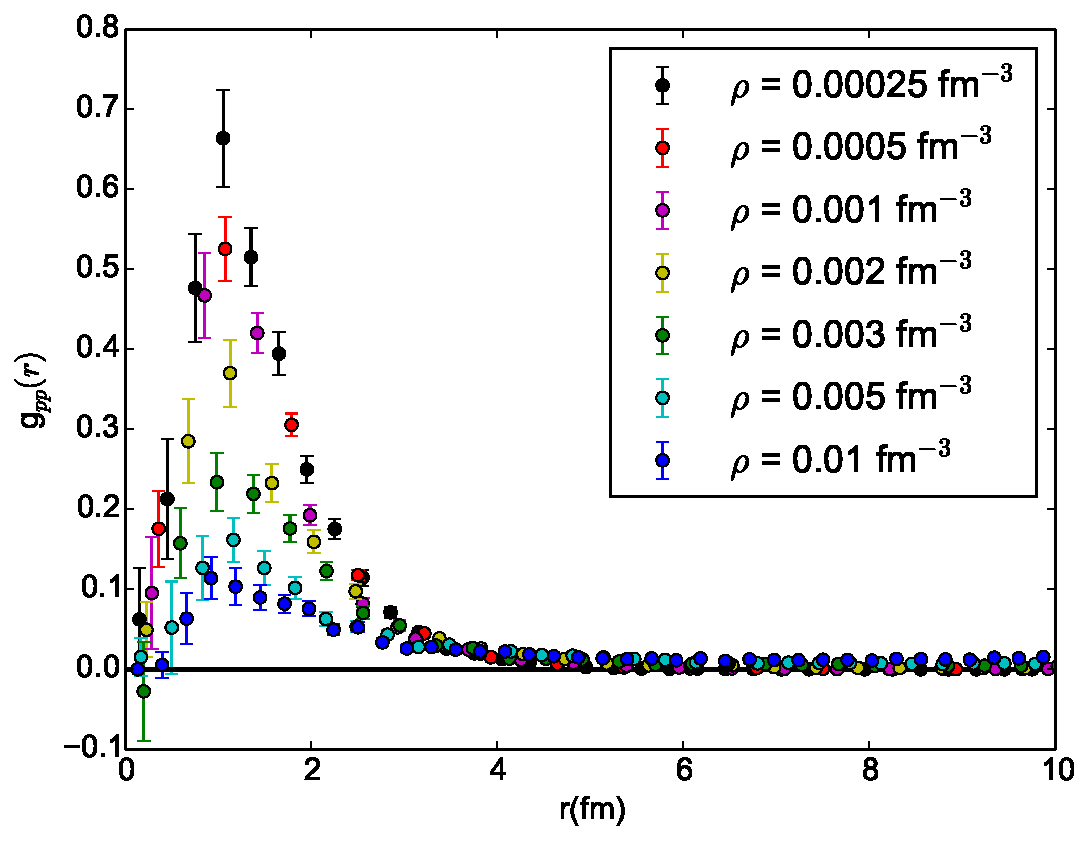
\includegraphics[width=0.7\textwidth]{figures/gpp.pdf}
   \caption[Pair Correlations Functions, $g_{pp}$ That Give the Probability of Finding 2 Protons a Distance $r$ from Each Other. This Is Only Shown for a Few of the Densities Calculated to Keep the Figure Less Busy.]{Pair correlations functions, $g_{pp}$ that give the probability of finding 2 protons a distance $r$ from each other. This is only shown for a few of the densities calculated to keep the figure less busy.}
   \label{fig:gpp}
\end{figure}
It is clear to see that as the density decreases the probability of finding the 2 protons at a close distance to each other increases. This is consistent with the formation of an alpha particle. The opposite is true, that as the density increases the protons are more likely to be found separated at larger distances, indicating the dissipation of the alpha particle at high densities. This can be seen in Figure~\ref{fig:gpp_small} which is simply showing more detail to the high separation tail in Figure~\ref{fig:gpp}
\begin{figure}[h!]
   \centering
   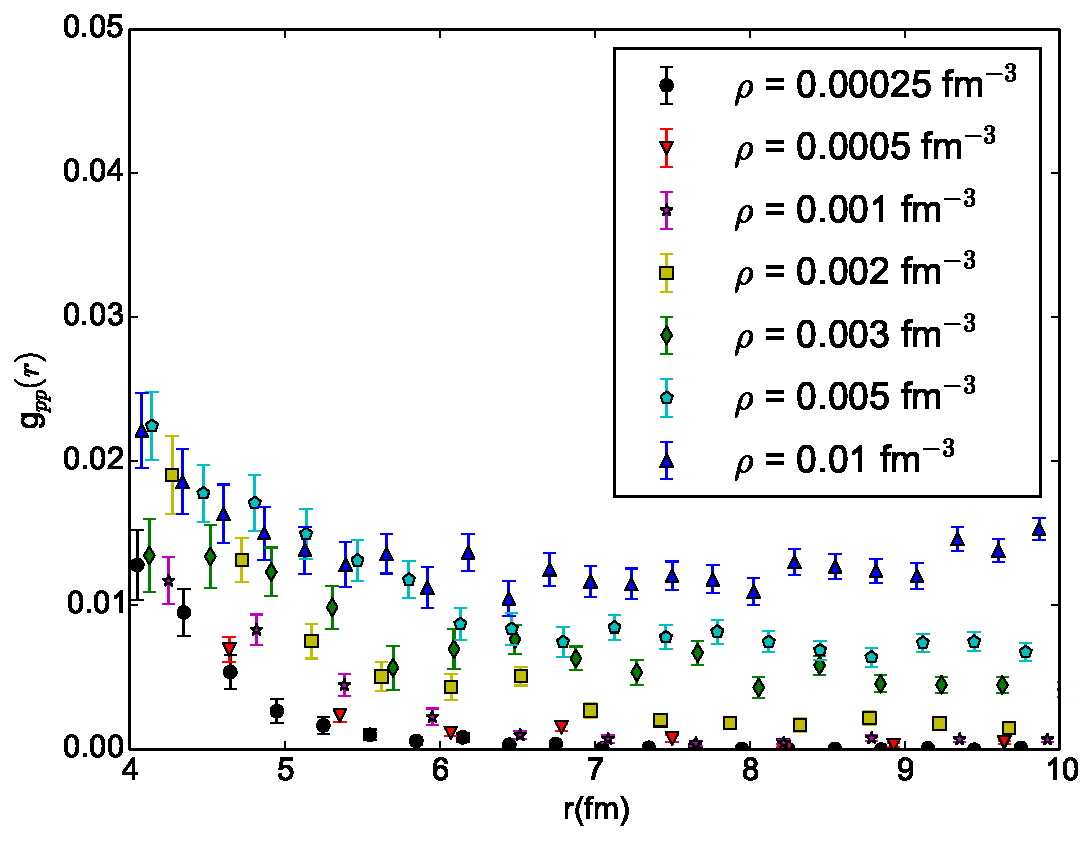
\includegraphics[width=0.7\textwidth]{figures/gpp_small.pdf}
   \caption[Large Separation Part of the Pair Correlations Functions $g_{pp}$ at Different Densities.]{Large separation part of the pair correlations functions $g_{pp}$ at different densities.}
   \label{fig:gpp_small}
\end{figure}

This provides good evidence that an alpha particle is forming at low densities. I have also calculated the pair distribution function for the alpha particle as calculated in the continuum, as opposed to the periodic box. In Figure~\ref{fig:gpp_compare} I have plotted this against the $g_{pp}$ pair distribution functions for the 14 neutrons with 2 protons at $\rho=0.00025$ fm$^{-3}$ as calculated with both linear and quadratic correlations. I have increased the resolution of the $g_{pp}$ calculation to show more detail.
\begin{figure}[h!]
   \centering
   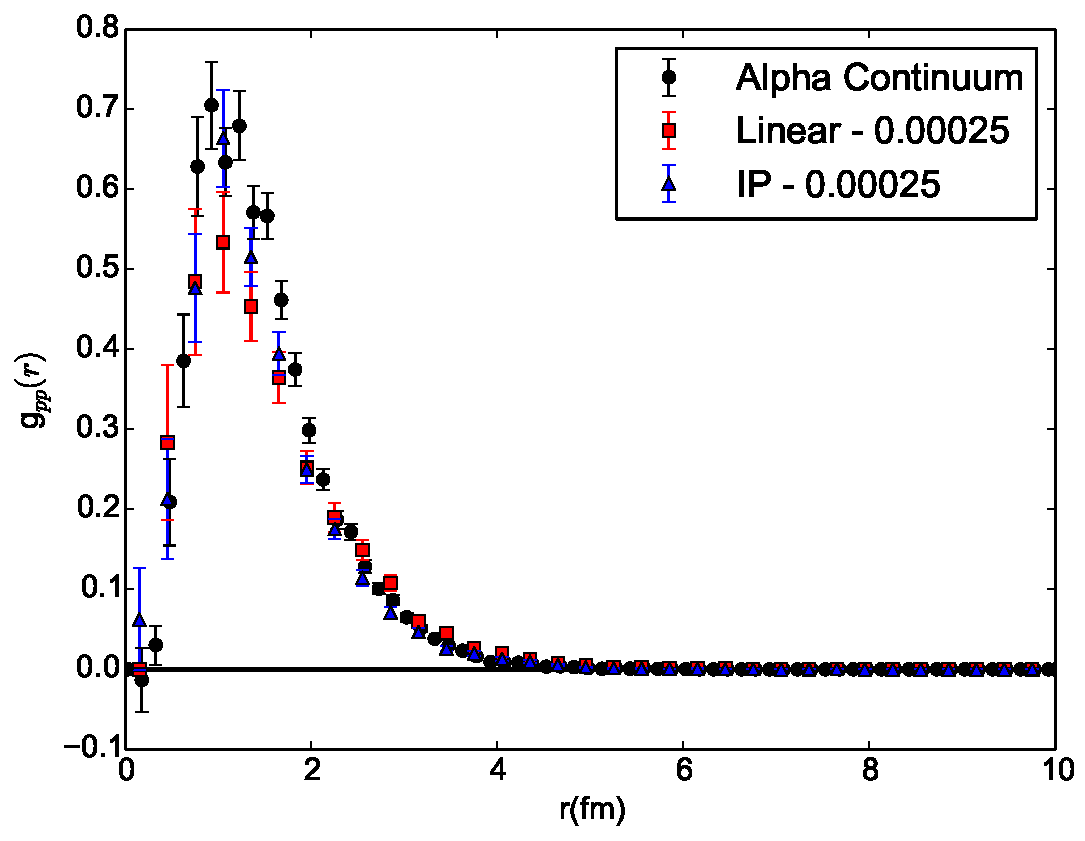
\includegraphics[width=0.7\textwidth]{figures/gpp_compare.pdf}
   \caption[Proton-proton Pair Distribution Functions Calculated in the Continuum Compared to the Calculation of 14 Neutrons and 2 Protons in a Periodic Box with $\rho=0.00025$ fm$^{-3}$. The $g_{pp}$ Calculations in the Box Have Increased Resolution Compared to Those in Earlier Plots to Show More Detail. Both Linear and IP Quadratic Correlations Were Used for the Calculations in a Box.]{Proton-proton pair distribution functions calculated in the continuum compared to the calculation of 14 neutrons and 2 protons in a periodic box with $\rho=0.00025$ fm$^{-3}$. The $g_{pp}$ calculations in the box have increased resolution compared to those in earlier plots to show more detail. Both linear and IP quadratic correlations were used for the calculations in a box.}
   \label{fig:gpp_compare}
\end{figure}
As was seen before both the linear and IP quadratic correlations seem to be forming an alpha particle, but the IP quadratic correlations provide a better fit to the pair correlation function of the alpha particle as calculated in the continuum, consistent with the energy calculations.

The energy can be split up into the different components of the AV6$'$ potential to study where the binding comes from and where the largest difference in the linear and quadratic correlations occurs. The alpha particle energy as split up into the AV6$'$ components for both linear and IP quadratic correlations is shown in Figure~\ref{fig:av6_alpha}.
\begin{figure}[h!]
   \centering
   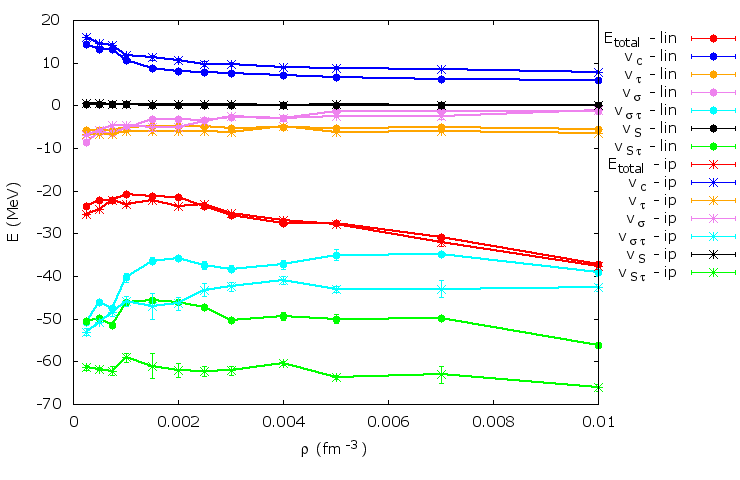
\includegraphics[width=0.9\textwidth]{figures/av6_alpha.png}
   \caption[Alpha Particle Energy as Calculated with Equation~\ref{equ:alphaenergy14n2p} for Each Piece of the AV6$'$ Potential for Both Linear and IP Quadratic Correlations.]{Alpha particle energy as calculated with Equation~\ref{equ:alphaenergy14n2p} for each piece of the AV6$'$ potential for both linear and IP quadratic correlations.}
   \label{fig:av6_alpha}
\end{figure}
The spin-isospin $\sigma\tau$ and tensor-isospin $S\tau$ operators from one-pion exchange are the operators most effected by the additional correlations in the improved wave function. In addition, the spin-isospin operators is fairly constant at high densities, but decreases for low densities, indicating that it is partially responsible for the alpha particle formation at low densities. This is expected as one-pion exchange is responsible for the long range binding of nuclei.
